% #############################################################################
% This is Chapter 2
% !TEX root = ../main.tex
% #############################################################################
\fancychapter{Related Work and Baseline SoC Selection}
\label{chap2:platform_foundation}



% #############################################################################
\section{SRAM-Based FPGA Architecture}
\label{chap2:fpga_arch}

\acp{FPGA} are integrated circuits whose logic and interconnect can be programmed after manufacture. Unlike \acp{ASIC}, where the circuit topology is fixed during fabrication, an \ac{FPGA} implements a user-defined circuit by configuring a fabric of programmable resources \cite{Kastensmidt2006}. The dominant commercial technology stores this configuration in \ac{SRAM} cells, which makes the device fully reconfigurable but also sensitive to radiation, as discussed in \cref{chap2:radiation}.

An \ac{SRAM}-based \ac{FPGA} is organised around three main categories of programmable resources. \acp{CLB} are the basic computation units; each contains one or more \acp{LUT}, a set of \acp{FF}, and carry-chain logic. A $k$-input \ac{LUT} implements any combinational Boolean function of $k$ variables by storing $2^k$ output bits in a small \ac{SRAM} array, so any function can be mapped to it at configuration time. \acp{FF} inside the \ac{CLB} register intermediate results and pipeline data between clock cycles. Routing resources — programmable switch matrices and interconnect segments — connect \ac{CLB} outputs to \ac{CLB} inputs; each routing switch is controlled by one or more \ac{SRAM} bits. Additional hard blocks, including dedicated block \ac{SRAM} arrays, \ac{DSP} slices, \acp{PLL}, and high-speed transceivers, are distributed across the device.

All of these resources — which \ac{LUT} implements which function, which routing switches are closed, how the \ac{I/O} pads behave — are determined by the \emph{configuration memory}: a large \ac{SRAM} array that holds the complete bitstream loaded into the device at power-up. The configuration memory is not user-accessible during normal operation; it is written once at startup and then drives the logic and routing fabric continuously. A change to any bit in the configuration memory changes the implemented circuit.

This \ac{SRAM}-based approach contrasts with flash-based \acp{FPGA}, which use non-volatile cells immune to soft errors but are generally slower and less scalable, and antifuse \acp{FPGA}, which are one-time programmable and highly radiation-hard but cannot be reconfigured. The focus of this thesis is exclusively on \ac{SRAM}-based \acp{FPGA}, where configuration memory is both the largest \ac{SRAM} structure on the device and the most radiation-sensitive one.


% #############################################################################
\section{Radiation Effects and Single Event Upsets}
\label{chap2:radiation}

Electronics deployed in space or at high altitude are continuously exposed to energetic charged particles originating from cosmic rays, solar particle events, and particles trapped in planetary radiation belts \cite{Petersen2011}. When such a particle traverses a semiconductor device, it deposits energy through ionisation, generating electron-hole pairs along its track. If the collected charge at a memory node exceeds the cell's critical charge threshold, the stored bit may be involuntarily inverted. This transient, radiation-induced bit flip — not caused by permanent device damage but by the passage of a single particle — is called a \ac{SEU}.

A \ac{SEU} is a soft error: the device is not physically damaged, but the stored state is corrupted until it is overwritten or the device is reset. In sequential logic, a \ac{SEU} in a register or \ac{FF} may propagate through subsequent pipeline stages as an erroneous value, leading to incorrect computation that is difficult to predict or reproduce without knowing exactly which bit was flipped and at which clock cycle.

\ac{SRAM}-based \acp{FPGA} are particularly exposed to \acp{SEU} because their programmable fabric is implemented on a large array of \ac{SRAM} cells — the configuration memory — that encodes the entire programmed design, including \ac{LUT} equations, routing connections, and \ac{I/O} configurations \cite{Kastensmidt2006}. A \ac{SEU} in this array does not merely corrupt a data value: it alters the hardware circuit itself, changing the behaviour of the running design until the device is reconfigured. Because configuration memory is orders of magnitude larger than the register file, it is statistically the most likely target for radiation-induced bit flips in space-deployed \ac{FPGA} designs. User data memory (\acp{FF}, block memories, and distributed memories) is also exposed, but upsets there produce data errors rather than structural modifications to the programmed logic.

Protecting against these effects requires either preventing faults from reaching sensitive nodes (physical shielding or radiation-hardened devices), tolerating them in hardware or software (\acp{FTM}), or actively detecting and correcting them (scrubbing). This thesis focuses on hardware-based \acp{FTM} and their evaluation through controlled \ac{FI}.



% #############################################################################
\section{Fault Injection Background}
\label{chap8:fi_background}

\ac{FI} techniques can be classified by the mechanism used to introduce faults \cite{Hsueh1997}. Simulation-based \ac{FI} modifies a hardware model at \ac{RTL} or gate level and observes the simulated response; it is accurate but does not capture implementation-specific timing and layout effects. Physical irradiation exposes real hardware to a particle beam or radiation source; it is the most realistic method but requires specialised facilities and is not easily reproducible. Emulation-based \ac{FI} uses a physical device — typically an \ac{FPGA} — and exploits its configuration interfaces or dedicated on-chip hardware to inject faults at runtime, combining hardware-accurate behaviour with controllability and repeatability. This work adopts emulation-based \ac{FI}.

\ac{FI} is the deliberate perturbation of a running system by provoking bit-flips in its memory elements, used to observe how faults propagate through the architecture and how detection, recovery, and masking mechanisms behave. \ac{FI} allows \acp{SEU} to be emulated without relying on particle beams or in-flight tests, enabling controlled and repeatable validation of \acp{FTM}.

% -------------------------------------------------------------
\subsection{Memory Types and Fault Targets}
\label{chap8:fi_targets}

\ac{SRAM}-based \acp{FPGA} contain multiple memory types that may be affected by \acp{SEU} \cite{PG187,Kastensmidt2006}. Listed in order of decreasing size — and therefore decreasing probability of being hit by a random upset — they are as follows.

Configuration memory stores the programmed configuration of the device, defining \ac{LUT} equations, routing connections, and \ac{I/O} behaviour. An upset here alters the implemented circuit rather than merely corrupting data, making it both the most structurally significant and statistically the most probable fault target.

Block memory provides large on-chip data storage, with bits clustered into dedicated physical blocks distributed across the device.

Distributed memory provides medium-capacity data storage using \ac{LUT}-based \ac{SRAM} elements within \acp{CLB}.

Flip-flops are the most common state elements in synchronous designs, used for pipelining, finite-state machines, and counters. They represent the smallest \ac{SRAM} area on the device.

Of these, configuration memory and registers/\acp{FF} are the two types targeted by the \ac{FI} tool developed in this work. Configuration-memory injection uses Xilinx's \ac{SEM} \ac{IP} for bit-level fault injection and the \ac{ACME} algorithm for module-level address selection, both described in the following subsections.




% -----------------------------------
\subsection{SEM IP to Execute Injections}
\label{chap8:fi_sem_theory}

Configuration-memory injections are executed using Xilinx's \ac{SEM} \ac{IP}, an on-chip controller that monitors and mitigates soft errors in \ac{FPGA} configuration memory. \ac{SEM} interacts with the configuration system through the \ac{ICAP}, which provides read and write access to configuration frames, using the device's built-in error-detection hardware to observe and correct configuration-memory errors.

In addition to its internal configuration connections, \ac{SEM} exposes multiple interfaces: a monitor interface (ASCII command console), a status interface (state, flags, heartbeat), optional \ac{ICAP} arbitration signals (for systems that share \ac{ICAP}), and optional external-memory support for error classification data storage.
The \ac{IP} can be configured in multiple modes: Mitigation and Testing, Mitigation Only, Detect and Testing, Detect Only, Emulation, and Monitoring Only. In this work, \ac{SEM} is instantiated in Mitigation and Testing mode with error classification disabled. Mitigation and Testing enables both continuous mitigation and controlled fault injection, while the detect-only variants restrict the controller to reporting behaviour. \ac{SEM}'s mitigation and correction features are not used in this work.
The system's behaviour changes with its current state in \ac{SEM}'s \ac{FSM}, displayed in \cref{fig:sem_state}, described in \cref{tab:sem_state_codes}, and controlled via commands listed in \cref{tab:sem_cmds_most_used}.

\begin{figure}[h]
  \centering
  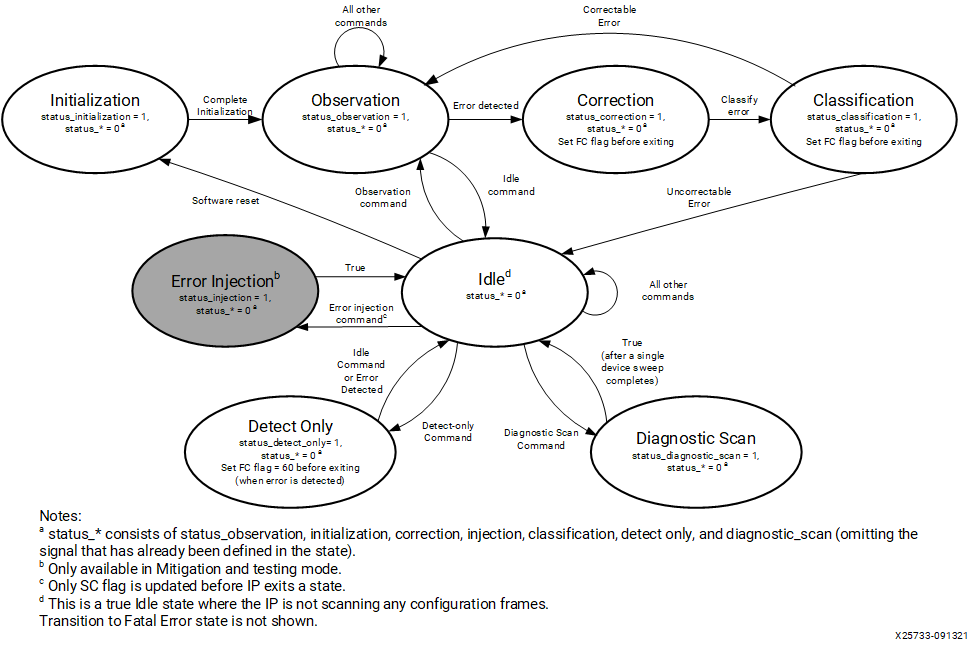
\includegraphics[width=0.88\linewidth]{Images/SEM_State_Machine.png}
  \caption{SEM state transition diagram for mitigation modes \cite{PG187}.}
  \label{fig:sem_state}
\end{figure}

\begin{table}[h]
\centering
\begin{tabularx}{\textwidth}{|l|l|X|}
\hline
Report & State & Meaning in practice \\
\hline
\hline
\texttt{SC 01} & Initialization & Startup sequence: configuration interfaces are checked and the controller is prepared to operate. \\
\hline
\texttt{SC 00} & Idle & Scanning is stopped. The controller accepts injection commands and status queries. The prompt becomes \texttt{I>}. \\
\hline
\texttt{SC 02} & Observation & Configuration continuous scanning is active. In mitigation modes, detected errors trigger correction. The prompt becomes \texttt{O>}. \\
\hline
\texttt{SC 04} & Correction & A configuration-memory error was detected and the controller is performing a correction cycle. \\
\hline
\texttt{SC 08} & Classification & Optional essential-bit classification step. When disabled, the controller may still pass through this state but does not fetch essential-bit data. \\
\hline
\texttt{SC 10} & Injection & An injection command is being executed. After the injected bit flip is applied, the controller returns to Idle. \\
\hline
\texttt{SC 1F} & Fatal error & Controller halted; the device typically requires reconfiguration. \\
\hline
\end{tabularx}
\caption{SEM state codes reported through the monitor interface (summary).}
\label{tab:sem_state_codes}
\end{table}


\begin{table}[h]
\centering
\begin{tabularx}{\textwidth}{|l|l|X|}
\hline
Command & Typical state & Effect on SEM \\
\hline
\hline
\texttt{I} & Observation or Idle & Forces the controller into Idle (\texttt{SC 00}). This is the injection-accepting state. \\
\hline
\texttt{O} & Idle or Observation & Forces the controller into Observation (\texttt{SC 02}) to resume scanning. \\
\hline
\texttt{S} & Idle or Observation & Prints a status summary (state, flags, maximum frame count, and related fields) and returns to the current prompt. \\
\hline
\texttt{N <addr>} & Idle & Performs a single configuration-bit injection. SEM reports \texttt{SC 10} (Injection) and then returns to Idle (\texttt{SC 00}). \\
\hline
\end{tabularx}
\caption{Most used SEM monitor commands. }
\label{tab:sem_cmds_most_used}
\end{table}

The N injection command flips exactly one configuration bit at the specified address. In UltraScale devices, the monitor expects an 11-digit hexadecimal value that encodes the injection location (including frame addressing plus the word and bit position inside the frame).
A typical injection sequence is shown in \cref{lst:sem_injection_flow}. The controller, currently on Idle, receives the injection and the bit flip is issued. The controller is then returned to Observation so that scanning (and, if enabled, correction) can proceed.

\begin{lstlisting}[float=h,caption={Typical \ac{SEM} monitor flow for one configuration injection (UltraScale format shown).},label={lst:sem_injection_flow}]
I> N C000A098000
SC 10
SC 00
I> O
SC 02
O>
\end{lstlisting}


% -----------------------------------
\subsection{ACME to Point Injections}
\label{chap8:fi_acme_theory}

\ac{SEM} injects faults by targeting an exact configuration-bit address, chosen from millions of possible addresses in an \ac{FPGA}. If addresses are selected uniformly at random, most injections land in unused or irrelevant configuration space, so the probability of affecting implemented logic is low. \ac{ACME} mitigates this problem by restricting injections to useful targets using an \ac{EBD} file that lists essential configuration bits, and a floorplanned region (pblock) that bounds the target module.

An \ac{EBD} file can be automatically generated through Vivado, and compresses the total board addresses into the addresses that actually contain configuration data. A pblock is a rectangular region placed at a fixed physical location on the device, defined in Vivado floorplan coordinates. In the Vivado flow, the user can force hardware modules to be confined to a pblock's borders, ensuring that injections within the pblock's range will land on those hardware modules.
The \ac{ACME} algorithm can then map pblock physical coordinates to the corresponding configuration-frame address range in the \ac{EBD} file. The published algorithm needs to be adapted for every target device, because the mapping constants are device-specific and must be calibrated for each board.


\ac{ACME} starts by converting the pblock bounds into an estimated interval of \ac{EBD} lines. The pblock is provided as a rectangle in floorplan coordinates, while the \ac{EBD} file is organised by line number. Therefore, \ac{ACME} first estimates which \ac{EBD} lines may contain essential bits from the selected physical region. For each clock region (a vertical tile band of the \ac{FPGA} fabric), \ac{ACME} uses a linear approximation between the relevant floorplan coordinate ($u$) and the corresponding \ac{EBD} line number ($\widehat{\ell}_{cr}$), as shown in \cref{eq:acme-line-map}. The constants $m_{cr}$ and $b_{cr}$ are device-specific parameters defined for each clock region.

\begin{equation}
\widehat{\ell}_{cr}(u) = m_{cr}u + b_{cr}
\label{eq:acme-line-map}
\end{equation}

The pblock bounds are evaluated with \cref{eq:acme-line-map}. When the pblock intersects more than one clock region, the mapping is applied to each affected region. \ac{ACME} then takes the lowest and highest estimated line numbers and rounds them outward, as shown in \cref{eq:acme-line-window}.

\begin{equation}
\ell_{\min} =
\left\lfloor
\min_{k}\ \widehat{\ell}_{cr(k)}(u_k)
\right\rfloor,
\qquad
\ell_{\max} =
\left\lceil
\max_{k}\ \widehat{\ell}_{cr(k)}(u_k)
\right\rceil
\label{eq:acme-line-window}
\end{equation}

The interval between $\ell_{\min}$ and $\ell_{\max}$ defines the \ac{EBD} line window used by \ac{ACME}. This step does not select the final essential bits. It only limits the search to the part of the \ac{EBD} file that can correspond to the target pblock.

The second step is to convert each essential bit of the target region into the tuple expected by \ac{SEM}, \{LA, WD, BT\}, where LA is a linear frame address, WD is the word index inside that frame, and BT is the bit index inside that 32-bit word. Since an \ac{EBD} file is an ASCII file with 32 characters per line — each character encoding one configuration bit as \texttt{`0'} or \texttt{`1'} — each line represents one 32-bit word of configuration data. Let $L$ be the (0-based) \ac{EBD} line index after skipping the file header and padding lines, and let $p$ be the character position of a `1' in that line (with $p=0$ at the leftmost character and $p=31$ at the rightmost character). Using the words-per-frame constant $W_f$ (device-dependent), the address fields can be obtained as shown in \cref{eq:acme_ebd_to_lawdbt}.

\begin{equation}
LA = \left\lfloor \frac{L}{W_f} \right\rfloor - 1,
\qquad
WD = L \bmod W_f,
\qquad
BT = 31 - p.
\label{eq:acme_ebd_to_lawdbt}
\end{equation}

The resulting list of packed configuration \{LA, WD, BT\} addresses can be used directly by the \ac{SEM} injection command stream, enabling injections that land on essential bits of the selected module rather than across the full device. 
In this work, \ac{ACME}-style expansion was implemented for the Basys3 and the KCU105 (XCKU040) boards \cite{basys3,xcku040}.



% #############################################################################
\section{Fault Tolerance Mechanisms}
\label{chap2:ftms}

\acp{FTM} are used to detect, mask, or correct faults, reducing their effect on system behaviour. They can be implemented in software or hardware, but this work focuses on hardware-based \acp{FTM}. This section introduces the mechanisms referenced or used throughout this thesis.

The handling of faults in a system can be characterised by the fault-error-failure chain: a \emph{fault} is the hypothesised root cause of an error, an \emph{error} is the incorrect system state that may lead to a failure, and a \emph{failure} occurs when the delivered service deviates from its specification \cite{Avizienis2004}. \acp{FTM} interrupt this chain at different points: \emph{detection} mechanisms identify errors before they propagate to a failure; \emph{masking} mechanisms absorb the fault and maintain correct output without explicit detection; and \emph{recovery} mechanisms restore the system to a correct state after an error has been detected. The following mechanisms, drawn from \cite{Kastensmidt2006} and the references therein, are referenced or implemented in this thesis.

Checksum \emph{(detection)} mechanisms add redundant check information to a data word or stored value. The check value is computed before storage or transmission and verified when the protected value is read, received, or used. If the recomputed check value does not match the stored one, the mechanism reports an error. Simple checksum mechanisms cannot detect an even number of simultaneous bit flips.

\ac{ECC} \emph{(detection and recovery)} expands on Checksum by using multiple check bits to detect and locate errors. For a 64-bit word, seven check bits can detect and correct a single-bit error and detect two-bit errors \cite{Hamming1950}.

Dual-Core Lockstep \emph{(detection)} runs a shadow instance of the core using delayed inputs, then compares its outputs against delayed main-core outputs. The delay ensures that a transient fault affecting one core at a given cycle does not simultaneously corrupt the other. A mismatch reports an error, but the mechanism cannot determine which output is correct \cite{ibex}.

Shadow \acp{CSR} \emph{(detection)} protect \acp{CSR} by keeping duplicated or bitwise-complemented copies of them. Glitches or corruption that break the relation between the main and shadow values trigger an alert \cite{ibex}.

An M-of-N system \emph{(masking)} implements redundancy. A block is replicated \(N\) times, and a voter accepts an output only when at least \(M\) replicas agree. With strict majority, \(M=\lfloor N/2 \rfloor+1\), the system can mask faults while most replicas remain correct. If no value reaches the required agreement, the mechanism reports an uncorrectable error \cite{Lyons1962}.

Scrubbing \emph{(recovery)} restores corrupted stored data after a correctable error is detected. In a redundant system, the accepted value can be written back into replicas or storage elements that disagree with it, preventing corrected faults from remaining stored and contributing to later failures. In \ac{SRAM}-based \acp{FPGA}, scrubbing also refers to periodically refreshing configuration memory frames to correct accumulated \acp{SEU} before they compound.

Self-testing \emph{(detection)} checks a block by applying predefined inputs and comparing the produced outputs with known results. These tests can be executed during idle periods or interleaved periodically with normal operation.




% #############################################################################
\section{State of the Art on Fault Tolerance Testing Platforms}
\label{chap2:existing_tools}

The lack of complete \ac{FT}/\ac{FI} platforms noted in \cref{chap1:motivation} is further illustrated in \cref{tab:fi_platforms_gap}, which compares state-of-the-art platforms according to the features needed to develop and test \acp{FTM}. Full \ac{RTL} shows whether the platform provides a modifiable hardware implementation required for \ac{FTM} integration. \ac{FT} Interface shows whether \acp{FTM} can be integrated and observed without building all fault signalling from scratch. Memory Types shows whether available \ac{FI} can cover the relevant \ac{FPGA} areas, including configuration memory and register/\ac{FF} memory. Readable \ac{UI} shows whether experiments can be defined through a user-facing configuration instead of per-run code edits. \ac{FI} Setup shows whether injection time and target selection can be reused across campaigns. Metrics shows whether \ac{FT}, performance, and hardware-cost results are extracted in a comparable form. The entries use Yes, Partial, and No to indicate whether each point is provided as part of an integrated workflow; Partial in the Memory Types column indicates that only a subset of the relevant memory types is covered.


\begin{table}[h]
\centering
\scriptsize
\setlength{\tabcolsep}{1.6pt}
\renewcommand{\arraystretch}{1.15}
\resizebox{\textwidth}{!}{%
\begin{tabular}{|p{0.18\textwidth}|c|c|c|c|c|c|}
\hline
\ac{FT}/\ac{FI} Platform &
Full \ac{RTL} &
\ac{FT} Interface &
Memory Types &
Readable \ac{UI} &
\ac{FI} Setup &
Metrics \\
\hline
\hline
Ruano \cite{ruano2021_fi_emulation} &
No & No & Partial & Partial & No & Partial \\
\hline
Critical bits \cite{mdpi2020_critical_bits} &
Partial & No & Partial & Partial & Partial & Partial \\
\hline
DPR FI \cite{wilson2021_dpr_fi} &
Partial & No & Partial & No & Partial & Partial \\
\hline
VeeR regs \cite{leon2024_veer_eh1_fi} &
Partial & No & Partial & No & No & Partial \\
\hline
Chiffre \cite{chiffre2018} &
No & No & Partial & Partial & Partial & No \\
\hline
Nail \cite{nail2025} &
No & No & Partial & Yes & Partial & No \\
\hline
ARCHIE \cite{archie} &
No & No & Partial & Yes & Partial & Partial \\
\hline
FEAR-V \cite{accellera_qemu_fea} &
No & No & Partial & Yes & Partial & Partial \\
\hline
QEFIRA \cite{qefira2024} &
No & Partial & Partial & Yes & Partial & Partial \\
\hline
InjectV \cite{injectv2025} &
No & No & Partial & Yes & Partial & Partial \\
\hline
CHAOS \cite{chaos2026} &
No & No & Partial & Partial & Partial & Partial \\
\hline
\hline
\ac{Fatori-V} &
Yes & Yes & Yes & Yes & Yes & Yes \\
\hline
\end{tabular}%
}
\caption{Comparison of state-of-the-art \ac{FT}/\ac{FI} platforms to test and develop \acp{FTM}.}
\label{tab:fi_platforms_gap}
\end{table}


\ac{FPGA} flows based on configuration memory injection, such as Ruano, Critical Bits, and DPR FI, cover configuration faults but not register/\ac{FF} injection. VeeR regs, Chiffre, and Nail cover register/\ac{FF} \ac{FI} but do not merge it with \ac{FPGA} configuration memory \ac{FI} in the experiments. Virtual-platform tools, such as ARCHIE, FEAR-V, QEFIRA, InjectV, and CHAOS, only provide campaign execution and logging in QEMU or gem5 environments, and lack \ac{FI} coverage across multiple memory types, implementation-level hardware cost reporting, and support for integrating new \ac{FTM} implementations. Across these groups, the main limitations are the lack of a complete \ac{SoC} workflow for integrating and comparing multiple \acp{FTM}, limited support for reusable \ac{FI} campaigns (temporal and spatial fault distributions), and result extraction often restricted to fault outcomes instead of comparable \ac{FT}, performance and hardware-cost metrics. \ac{Fatori-V} was developed to address these gaps, as described from \cref{chap3:fatori-v} onward.








% #############################################################################
\section{Comparative Analysis of RISC-V SoCs}
\label{chap2:analysis}


\ac{RISC-V} is an open, royalty-free \ac{ISA} originally developed at UC Berkeley, defined around a small base integer instruction set with a set of optional standard extensions \cite{riscv-isa}. Its open specification and the resulting ecosystem of open-source soft-processor implementations make it attractive for research and for space applications where hardware auditability and customisability are important. All candidates surveyed in this section are \ac{RISC-V} soft-processor implementations that can be deployed on \ac{SRAM}-based \acp{FPGA}.

\ac{Fatori-V} required an existing open-source \ac{RISC-V} \ac{RTL} baseline that supported \ac{RTL} modification, \ac{FTM} integration, software execution, and \ac{FPGA} implementation. This section compares candidate state-of-the-art \acp{SoC} against the baseline selection criteria.

The surveyed candidates were CVA6 \cite{CVA6}, a 64-bit Linux-capable core; CV32E40P \cite{cv32e40p}, a 32-bit embedded core from the PULP lineage; Ibex \cite{ibex}, a 32-bit embedded core with build-time configuration and native \ac{FT} support; PicoRV32 \cite{picorv32}, a small multi-cycle core with minimal \ac{SoC} examples; Rocket Chip \cite{rocket_chip}, a Chisel-based generated \ac{SoC}; VeeR EL2 through VeeRwolf \cite{VeeRwolf}, a 32-bit embedded core with a runnable \ac{SoC}, debug tools, and course material; and VexRiscv \cite{vexriscv}, a SpinalHDL-generated configurable core. \Cref{tab:candidate_comparison_fullcriteria} reports the comparison using public documentation, direct inspection of the source code, and reported implementation data. Documentation is graded from 0 to 10. Readability, workflow, \ac{FT} infrastructure, development access, and community activity are qualitative. Published area and performance values are supporting indicators because they may come from different configurations and devices.



\begin{table}[h]
\centering
\scriptsize
\setlength{\tabcolsep}{1.1pt}
\renewcommand{\arraystretch}{1.22}
\begin{tabular}{|
>{\raggedright\arraybackslash}p{0.085\textwidth}|
>{\centering\arraybackslash}p{0.030\textwidth}|
>{\raggedright\arraybackslash}p{0.125\textwidth}|
>{\raggedright\arraybackslash}p{0.125\textwidth}|
>{\raggedright\arraybackslash}p{0.130\textwidth}|
>{\raggedright\arraybackslash}p{0.085\textwidth}|
>{\raggedright\arraybackslash}p{0.125\textwidth}|
>{\raggedright\arraybackslash}p{0.120\textwidth}|
>{\raggedright\arraybackslash}p{0.08\textwidth}|
}
\hline
Core &
Doc. &
Readability and Modification &
Workflow &
FT Infrastructure &
Dev. Access &
Min. Hardware Cost &
Max. Performance &
Community \\
\hline
\hline
CVA6 &
8 &
Low, complex core &
High, Linux-capable &
Small &
No &
--- &
3.1\,CoreMark/\newline MHz* \cite{CVA6_maxperf} &
High \\
\hline
CV32E40P &
7 &
High, clean SV &
High, MCU platform &
None &
No &
40 kG* (conf V1) \cite{CV32E40P_minhw} &
3.19\,CoreMark/\newline MHz* \cite{CV32E40P_maxperf} &
High \\
\hline
Ibex &
8 &
Very High, modular code &
Medium, simple demo system &
Full, 7+ FTMs + FT Interface &
No &
16.85\,kGE* (micro) \cite{ibex} &
3.13\,CoreMark/\newline MHz* (maxperf) \cite{Ibex_maxperf} &
Very high \\
\hline
PicoRV32 &
4 &
Very High, small RTL &
Medium, PicoSoC included &
None &
Local SoC Implementation &
\(\sim\)750 LUT* \newline (Xilinx 7-series) \cite{PicoRV32_minhw} &
0.40\,CoreMark/\newline MHz* \cite{PicoRV32_maxperf} &
High \\
\hline
Rocket Chip &
6 &
Very Low, generator heavy &
Very High, Chipyard flow &
Small &
No &
--- &
2.108\,CoreMark/\newline MHz* (Rocket) \cite{RocketChip_maxperf} &
Very high \\
\hline
VeeR EL2 &
10 &
Medium, SoC coupled &
Very High, custom debug tools &
Medium*, Data/RF ECC, Lockstep &
Previous work &
--- &
3.6\,CoreMark/\newline MHz* \cite{VeeR_EL2_maxperf} &
High \\
\hline
VexRiscv &
6 &
Low, generator workflow &
Medium, many integrations &
None &
Local SoC Implementation &
504 LUT, 505 FF* \newline (small) \cite{VexRiscv_minhw} &
1.57\,DMIPS/\newline MHz* \cite{VexRiscv_maxperf} &
High \\
\hline
\end{tabular}
\caption{Comparison of open-source \ac{RISC-V} candidates against the baseline selection criteria. Values marked with * come from specific published configurations. VexRiscv performance is reported in DMIPS/MHz as no CoreMark figure was found.}
\label{tab:candidate_comparison_fullcriteria}
\end{table}


The comparison reduced the choice to Ibex and VeeR EL2. The remaining candidates were discarded because they either lacked native \ac{FT} support, depended on generator-based flows, targeted larger application-class systems, or provided limited \ac{SoC} infrastructure. Ibex offered stronger \ac{FT} support, with multiple native \acp{FTM}, a defined error interface, alert classification, compact \ac{RTL}, clear module boundaries, well-defined integration interfaces, and build-time configurability. Its main drawback was the need to select and integrate an external \ac{SoC} workflow, since its available demo systems are lightweight and the baseline is mostly core-centric outside the OpenTitan security project, which is not suitable as a general-purpose baseline.

VeeR EL2 through VeeRwolf offered a more complete starting workflow, with guided labs, examples, demos, board tutorials, reference documentation, a runnable \ac{SoC}, debug tools, and prior group experience with the platform. Its main drawbacks were stronger \ac{SoC} coupling, a larger codebase, fewer native \acp{FTM}, and less unified fault handling. VeeR EL2 through VeeRwolf was selected as the first \ac{RTL} backbone for \ac{Fatori-V} because the available workflow was expected to reduce early integration risk. The main risk was that, if the guides and tools did not support the required \ac{RTL} changes, the coupled codebase and larger \ac{FTM} implementation load could cause major delays, as discussed in \cref{chap4:el2}.

% #############################################################################
\section{Summary}
\label{chap2:summary}

This chapter established the background required for the remainder of the thesis: the \ac{SRAM}-based \ac{FPGA} architecture and radiation environment that motivate fault injection, the injection and targeting techniques used in this work, the fault tolerance mechanisms evaluated, the gap in existing \ac{FT}/\ac{FI} platforms, and the selection of VeeR EL2 as the initial \ac{RISC-V} baseline. \Cref{chap3:fatori-v} presents the overall design of the \ac{Fatori-V} platform built on top of this foundation.

